\let\negmedspace\undefined
\let\negthickspace\undefined
\documentclass[journal,12pt,twocolumn]{IEEEtran}
\usepackage{gensymb}
\usepackage{amssymb}
\usepackage[cmex10]{amsmath}
\usepackage{amsthm}
\usepackage[export]{adjustbox}
\usepackage{bm}
\usepackage{longtable}
\usepackage{enumitem}
\usepackage{mathtools}
\usepackage[breaklinks=true]{hyperref}
\usepackage{listings}
\usepackage{color}                                            %%
\usepackage{array}                                            %%
\usepackage{longtable}                                        %%
\usepackage{calc}                                             %%
\usepackage{multirow}                                         %%
\usepackage{hhline}                                           %%
\usepackage{ifthen}                                           %%
\usepackage{lscape}     
\usepackage{multicol}
% \usepackage{enumerate}
\DeclareMathOperator*{\Res}{Res}
\renewcommand\thesection{\arabic{section}}
\renewcommand\thesubsection{\thesection.\arabic{subsection}}
\renewcommand\thesubsubsection{\thesubsection.\arabic{subsubsection}}
\renewcommand\thesectiondis{\arabic{section}}
\renewcommand\thesubsectiondis{\thesectiondis.\arabic{subsection}}
\renewcommand\thesubsubsectiondis{\thesubsectiondis.\arabic{subsubsection}}
\hyphenation{op-tical net-works semi-conduc-tor}
\def\inputGnumericTable{}                                 %%
\lstset{
frame=single, 
breaklines=true,
columns=fullflexible
}
\begin{document}
\newtheorem{theorem}{Theorem}[section]
\newtheorem{problem}{Problem}
\newtheorem{proposition}{Proposition}[section]
\newtheorem{lemma}{Lemma}[section]
\newtheorem{corollary}[theorem]{Corollary}
\newtheorem{example}{Example}[section]
\newtheorem{definition}[problem]{Definition}
\newcommand{\BEQA}{\begin{eqnarray}}
\newcommand{\EEQA}{\end{eqnarray}}
\newcommand{\define}{\stackrel{\triangle}{=}}
\bibliographystyle{IEEEtran}
\providecommand{\mbf}{\mathbf}
\providecommand{\pr}[1]{\ensuremath{\Pr\left(#1\right)}}
\providecommand{\qfunc}[1]{\ensuremath{Q\left(#1\right)}}
\providecommand{\sbrak}[1]{\ensuremath{{}\left[#1\right]}}
\providecommand{\lsbrak}[1]{\ensuremath{{}\left[#1\right.}}
\providecommand{\rsbrak}[1]{\ensuremath{{}\left.#1\right]}}
\providecommand{\brak}[1]{\ensuremath{\left(#1\right)}}
\providecommand{\lbrak}[1]{\ensuremath{\left(#1\right.}}
\providecommand{\rbrak}[1]{\ensuremath{\left.#1\right)}}
\providecommand{\cbrak}[1]{\ensuremath{\left\{#1\right\}}}
\providecommand{\lcbrak}[1]{\ensuremath{\left\{#1\right.}}
\providecommand{\rcbrak}[1]{\ensuremath{\left.#1\right\}}}
\theoremstyle{remark}
\newtheorem{rem}{Remark}
\newcommand{\sgn}{\mathop{\mathrm{sgn}}}
\providecommand{\abs}[1]{\left\vert#1\right\vert}
\providecommand{\res}[1]{\Res\displaylimits_{#1}} 
\providecommand{\norm}[1]{\left\lVert#1\right\rVert}
%\providecommand{\norm}[1]{\lVert#1\rVert}
\providecommand{\mtx}[1]{\mathbf{#1}}
\providecommand{\mean}[1]{E\left[ #1 \right]}
\providecommand{\fourier}{\overset{\mathcal{F}}{ \rightleftharpoons}}
%\providecommand{\hilbert}{\overset{\mathcal{H}}{ \rightleftharpoons}}
\providecommand{\system}{\overset{\mathcal{H}}{ \longleftrightarrow}}
	%\newcommand{\solution}[2]{\textbf{Solution:}{#1}}
\newcommand{\solution}{\noindent \textbf{Solution: }}
\newcommand{\cosec}{\,\text{cosec}\,}
\providecommand{\dec}[2]{\ensuremath{\overset{#1}{\underset{#2}{\gtrless}}}}
\newcommand{\myvec}[1]{\ensuremath{\begin{pmatrix}#1\end{pmatrix}}}
\newcommand{\mydet}[1]{\ensuremath{\begin{vmatrix}#1\end{vmatrix}}}
\numberwithin{equation}{subsection}
\makeatletter
\@addtoreset{figure}{problem}
\makeatother
\let\StandardTheFigure\thefigure
\let\vec\mathbf
\renewcommand{\thefigure}{\theproblem}
\def\putbox#1#2#3{\makebox[0in][l]{\makebox[#1][l]{}\raisebox{\baselineskip}[0in][0in]{\raisebox{#2}[0in][0in]{#3}}}}
     \def\rightbox#1{\makebox[0in][r]{#1}}
     \def\centbox#1{\makebox[0in]{#1}}
     \def\topbox#1{\raisebox{-\baselineskip}[0in][0in]{#1}}
     \def\midbox#1{\raisebox{-0.5\baselineskip}[0in][0in]{#1}}
\vspace{3cm}
\title{10th CBSE MATHEMATICS}
\author{ 2008-09
	\thanks{}
}
\maketitle
\newpage
\bigskip
\renewcommand{\thefigure}{\theenumi}
\renewcommand{\thetable}{\theenumi}
\section{Section A}
\renewcommand{\theequation}{\theenumi}
\begin{enumerate}[label=\thesection.\arabic*.,ref=\thesection.\theenumi]
\numberwithin{equation}{enumi}
\item Complete the missing entries in the following factor tree :\\
\begin{figure}[h!]
    \centering
    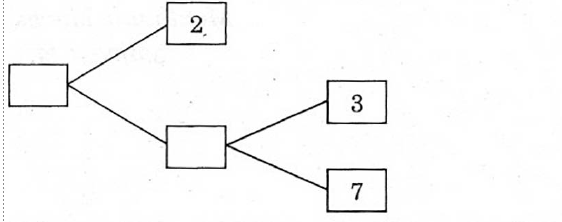
\includegraphics[width=0.5\columnwidth,center]{./fig/1.png}
	\caption{}
	\label{fig1}
 \end{figure}
\item If $(x+a)$ is a factor of $2x2+2ax+5x+10$, find $a$.\\
\item  Show that $x=-3$ is a solution of $x2+6x+9=0$.\\
\item The first term of an $A.P$. is $p$ and its common difference is $q$. Find its $10^{th}$ term. \\
\item If $\tan A=\frac{5}{12}$, find the value of $(\sin A+\cos A)\sec A$. \\
\item The lengths of the diagonals of a rhombus are $30 cm$ and $40 cm$. Find the side of the rhombus. \\
\item In Figure \ref{fig2}, $PQ||BC$ and $AP:PB=1:2$. Find $\frac{ar(\triangle APQ)}{ar(\triangle ABC)}$.\\
\begin{figure}[h!]
	\centering
    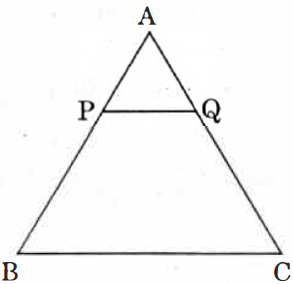
\includegraphics[width=0.5\columnwidth,center]{./fig/2.png}
    \caption{}
    \label{fig2}
\end{figure}
\item The surface area of a sphere is 616 $cm^2$. Find its radius.\\
\item A die is thrown once. Find the probability of getting a number less than $3$.\\  
\item Find the class marks of classes $10 -25$ and $35 -55$ . \\
\end{enumerate}
\section{Section B}
\renewcommand{\theequation}{\theenumi}
\begin{enumerate}[label=\thesection.\arabic*.,ref=\thesection.\theenumi]
\numberwithin{equation}{enumi}
\item Find all the zeros of the polynomial $x^4+x^3-34x^2-4x=120$, if two of its zeros are $2,-2$.\\
\item A pair of dice is thrown once. Find the probability of getting the same number on each dice. \\
\item If $\sec4A=\cosec(A-20\degree)$, where $4A$ is an acute angle, find the value of $A$.\\
\begin{align}
	\centering \vec{OR}\nonumber
\end{align}
In a ,$\triangle ABC$, right-angled at $C$, if $\tan A=\frac{1}{\sqrt{3}}$ , find the value of $\sin A \cos B+ \cos A \sin B$.\\
\item Find the value of $k$ if the points $(k, 3), (6, -2)$ and $(-3, 4)$ are collinear.\\
\item $E$ is a point on the side $AD$ produced of a $\parallel^{gm} ABCD$ and $BE$ intersects $CD$ at $F$. Show that $\triangle ABE \sim \triangle CFB$.
\end{enumerate}
\section{Section C}
\renewcommand{\theequation}{\theenumi}
\begin{enumerate}[label=\thesection.\arabic*.,ref=\thesection.\theenumi]
\numberwithin{equation}{enumi}
\item Use Euclid's Division Lemma to show that the square of any positive integer is either of the form $3m$ or $(3m + 1)$ for some integer $m$.\\ 
\item Represent the following pair of equations graphically and write the coordinates of pointswhere the lines intersect $y-axis:$\\
$x+3y=6$ \\
$2x-3y=12$ \\
\item For what value of $n$ are the $n^{th}$ terms of two A.P.'s $63, 65, 67,$ ... and $3, 10, 17$, ... equal ?\\
	\begin{align}
		\centering \vec{OR}\nonumber
	\end{align}
If m times the $m^{th}$ term of an $A.P$. is equal to $n$ times its $n^{th}$ term, find the $(m+n)^{th}$ term of the $A.P$.
\item In an $A,P$., the first term is $8$, $n^{th}$ term is $33$ and sum to first n terms is $123$. Find $n$ and $d$, the common difference.\\
\item Prove that: \\ $(1 + \cot A+ \tan A) (\sin A - \cos A) = \sin A \tan A - \cot A \cos A$.\\
	\begin{align}
		\centering \vec{OR}\nonumber
	\end{align}
Without using trigonometric tables, evaluate the following:\\
$2\frac{\cos58\degree}{\sin32\degree}-\sqrt{3}\frac{\cos38\degree \cosec52\degree}{\tan15\degree \tan60\degree \tan75\degree}$\\
\item If $P$ divides the join of $A(-2, -2) and B(2, -4)$ such that $\frac{AP}{AB}=\frac{3}{7}$, find the coordinates of $P$.\\
\item The mid-points of the sides of a triangle are $(3, 4), (4, 6)$ and $(5, 7)$. Find the coordinates· of the vertices of the triangle.\\
\item Draw a right triangle in which the sides containing the right angle are $5$ cm and $4$ cm. Construct a similar triangle whose sides are. $\frac{5}{3}$ times the sides of the above triangle.\\
\item Prove that a parallelogram circumscribing a circle is a rhombus.
\begin{align}
	\centering \vec{OR}\nonumber
\end{align}
In Figure \ref{fig3}, $AD\perp BC$. \\Prove that $AB^2+CO^2=B0^2+AC^2$.\\
\begin{figure}[h!]
	\centering
    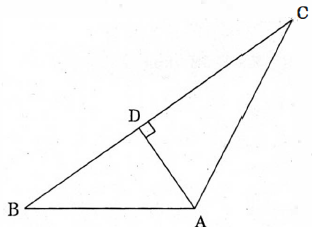
\includegraphics[width=0.5\columnwidth,center]{./fig/3.png}
	\caption{}
	\label{fig3}
\end{figure}
\item In Figure \ref{fig4}, ABC is a quadrant of a circle of radius $14 cm$ and a semi-circle is drawn with $BC$ as diameter. Find the area of the shaded region.
\begin{figure}[h!]
    \centering
    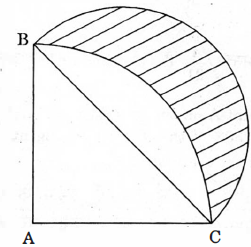
\includegraphics[width=0.5\columnwidth,center]{./fig/4.png}
    \caption{}
    \label{fig4}
\end{figure}
\end{enumerate}   
\section{Section D}
\renewcommand{\theequation}{\theenumi}
\begin{enumerate}[label=\thesection.\arabic*.,ref=\thesection.\theenumi]
\numberwithin{equation}{enumi}
\item A peacock is sitting on the top of a pillar, which is $9 m$ high. From a point $27 m$ away from the bottom of the pillar, a snake is coming to its hole at the base of the pillar. Seeing the snake the peacock pounces on it. If their speeds are equal, at what distance from the hole is the snake caught ?\\
	\begin{align}
		\centering \vec{OR}\nonumber
	\end{align}
The difference of two numbers is $4$. If the difference of their reciprocals $\frac{4}{21}$  is , find the two numbers. \\
\item The angle of elevation of an aeroplane from a point A on the ground is 60\degree. After a flight of $30$ seconds, the angle of elevation changes to 30\degree. If the plane is flying at a constant height of $3600 \sqrt{3} m$, find the speed, in km/hour, of the plane .\\
\item If a line is drawn parallel to one side of a triangle to intersect the other two sides in distinct points, prove that the other two sides are divided in the same ratio.\\
Using the above, prove the following :\\
In Figure \ref{fig5}, $AB\parallel DE$ and $BC \parallel EF$. Prove that $AC \parallel DF$.
\begin{figure}[h!]
	\centering
    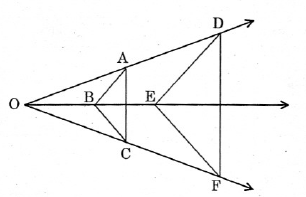
\includegraphics[width=0.5\columnwidth, center]{./fig/5.png}
    \caption{}
    \label{fig5}
\end{figure}
\begin{align}
\centering \vec{OR}\nonumber
\end{align}
Prove that the lengths of tangents drawn from an external point to a circle are equal. Using the above, prove the following : \\
$ABC$ is an isosceles triangle in which $AB = AC$, circumscribed about a circle, as shown in Figure \ref{fig6}. Prove that the base is bisected by the point of contact. \\
\begin{figure}[h!]
	\centering
    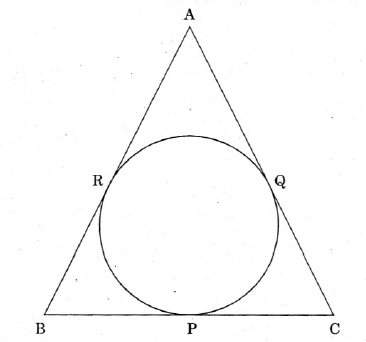
\includegraphics[width=0.5\columnwidth,center]{./fig/6.png}
    \caption{}
    \label{fig6}
\end{figure}
\item If the radii of the circular ends of a conical bucket, which is $16 cm$ high, are $20 cm$ and $8 cm$, find the capacity and total surface area of the bucket. (Use $\pi=\frac{22}{7}$)\\
\end{enumerate}
\begin{enumerate}
\item Find mean, median and mode of the following data :\\
\begin{center}
    \centering{
        \begin{tabular}{|p{3 cm}|p{3 cm}|}
        \hline
        Class & Frequency \\  
        \hline
            0-20  &  6  \\
            \hline
            20-40 &  8 \\
            \hline
            40-60  &  10 \\
            \hline
            60-80 &  12  \\
            \hline
            80-100  &  6   \\
            \hline
            100-120 &  5  \\
            \hline
            120-140  &  3   \\
        \hline
        \end{tabular}
   } \end{center}
\end{enumerate}
\end{document}
